\begin{pastexam}[label={px:df3-103-ds-01}]{地方三等資訊處理 103 年 第一題}
（申論；25 分）

給定一個權重圖（weighted graph）G(V, E) 如下圖所示。
\begin{itemize}[leftmargin=2.2em, nosep]
\item[㈠] 請用 Kruskal 演算法找出最小生成樹 MST(G) (minimum spanning tree)。請依序寫出加入此最小生成樹的
每一個邊。（5 分）
\item[㈡] 請用 Prim 演算法找出最小生成樹 MST(G)。若以 A 為起始點，請依序寫出加入此最小生成樹的每一個邊。
（5 分）
\item[㈢] 假設最小生成樹 MST(G) 已知。若在原圖 G(V, E) 中加入一個新的邊 $v_i$ - $v_j$ 且其權重為 $w$。請設計
一個 O(V) 的演算法，從已知的 MST(G) 中快速找出新圖的最小生成樹。請以文字敘述說明。（10 分）
\item[㈣] 請說明上一小題㈢的演算法為 O(V)。（5 分）
\end{itemize}
\begin{center}
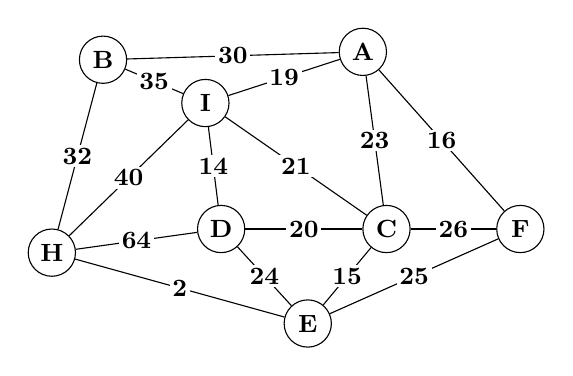
\begin{tikzpicture}[v/.style={circle,draw,minimum size=6mm,inner sep=0pt,font=\small\bfseries},
  lab/.style={font=\small\bfseries,fill=white,inner sep=1pt}]
\node[v] (B) at (1.2,0.95) {B};
\node[v] (A) at (4.5,1.05) {A};
\node[v] (I) at (2.5,0.4) {I};
\node[v] (H) at (0.55,-1.5) {H};
\node[v] (D) at (2.7,-1.2) {D};
\node[v] (C) at (4.8,-1.2) {C};
\node[v] (F) at (6.5,-1.2) {F};
\node[v] (E) at (3.8,-2.4) {E};
\draw (B) -- node[lab] {30} (A);
\draw (B) -- node[lab] {35} (I);
\draw (I) -- node[lab] {19} (A);
\draw (B) -- node[lab] {32} (H);
\draw (I) -- node[lab] {40} (H);
\draw (I) -- node[lab] {14} (D);
\draw (I) -- node[lab] {21} (C);
\draw (A) -- node[lab] {23} (C);
\draw (A) -- node[lab] {16} (F);
\draw (D) -- node[lab] {20} (C);
\draw (C) -- node[lab] {26} (F);
\draw (H) -- node[lab] {64} (D);
\draw (D) -- node[lab] {24} (E);
\draw (C) -- node[lab] {15} (E);
\draw (E) -- node[lab] {25} (F);
\draw (H) -- node[lab] {2} (E);
\end{tikzpicture}
\end{center}
\end{pastexam}

\begin{pastsoln}
答案：㈠ 依序 $(H,E)$ 2、$(I,D)$ 14、$(C,E)$ 15、$(A,F)$ 16、$(I,A)$ 19、$(D,C)$ 20、$(B,A)$ 30，總權重 $116$。
㈡ 依序 $(A,F)$ 16、$(A,I)$ 19、$(I,D)$ 14、$(D,C)$ 20、$(C,E)$ 15、$(E,H)$ 2、$(A,B)$ 30，同一棵樹。
㈢㈣ 在樹上找 $v_i$ 到 $v_j$ 的路徑，把路徑上最重的邊和新邊比較，較重的那條丟掉；$O(V)$。

圖有 $8$ 個頂點、$16$ 條邊，權重都不同，所以最小生成樹唯一（資結書定理~24.4），兩種演算法得到同一棵樹，
只是加入的順序不同。

\textbf{㈠ Kruskal}（資結書第~24.2~節）：邊由小到大檢查，不形成迴路就收。
\begin{center}
\begin{tabular}{ccl}
\toprule
邊 & 權重 & 結果 \\
\midrule
$(H,E)$ & 2 & 收 \\
$(I,D)$ & 14 & 收 \\
$(C,E)$ & 15 & 收；$\{C,E,H\}$ \\
$(A,F)$ & 16 & 收 \\
$(I,A)$ & 19 & 收；$\{A,D,F,I\}$ \\
$(D,C)$ & 20 & 收；$\{A,C,D,E,F,H,I\}$ \\
$(I,C)$ & 21 & 丟：$I$、$C$ 已連通 \\
$(A,C)$ & 23 & 丟 \\
$(D,E)$ & 24 & 丟 \\
$(E,F)$ & 25 & 丟 \\
$(C,F)$ & 26 & 丟 \\
$(B,A)$ & 30 & 收；全部連通，共 $7$ 條，結束 \\
\bottomrule
\end{tabular}
\end{center}
加入順序：$(H,E)$, $(I,D)$, $(C,E)$, $(A,F)$, $(I,A)$, $(D,C)$, $(B,A)$，總權重 $2 + 14 + 15 + 16 + 19 + 20 + 30 = 116$。

\textbf{㈡ Prim，從 A 開始}（資結書第~24.3~節）：每次選一端在樹內、一端在樹外的最輕邊。
\begin{center}
\begin{tabular}{lll}
\toprule
樹內的頂點 & 候選的最輕邊 & 加入 \\
\midrule
$A$ & $AF$ 16、$AI$ 19、$AC$ 23、$AB$ 30 & $(A,F)$ 16 \\
$A, F$ & $AI$ 19、$AC$ 23、$FE$ 25、$FC$ 26 & $(A,I)$ 19 \\
$A, F, I$ & $ID$ 14、$IC$ 21、$IB$ 35、$IH$ 40 & $(I,D)$ 14 \\
$A, F, I, D$ & $DC$ 20、$IC$ 21、$DE$ 24 & $(D,C)$ 20 \\
$A, F, I, D, C$ & $CE$ 15、$DE$ 24 & $(C,E)$ 15 \\
$A, F, I, D, C, E$ & $EH$ 2、$AB$ 30 & $(E,H)$ 2 \\
$A, F, I, D, C, E, H$ & $AB$ 30、$BH$ 32、$BI$ 35 & $(A,B)$ 30 \\
\bottomrule
\end{tabular}
\end{center}
（每一列只列出最輕的幾條候選。）加入順序：$(A,F)$, $(A,I)$, $(I,D)$, $(D,C)$, $(C,E)$, $(E,H)$, $(A,B)$，總權重同樣是 $116$。

\textbf{㈢ 演算法。} 設 $T$ 是原本的最小生成樹，新邊 $e = (v_i, v_j)$、權重 $w$。
\begin{enumerate}
\item 在 $T$ 上從 $v_i$ 做 DFS（或 BFS），記錄每個頂點的父節點，直到走到 $v_j$；沿父節點從 $v_j$ 往回走，
得到 $T$ 中 $v_i$ 到 $v_j$ 的唯一路徑 $P$。
\item 沿 $P$ 找出最重的邊 $f$，權重 $w_f$。
\item 若 $w < w_f$：新的最小生成樹是 $T - f + e$。 否則 $T$ 不變（$e$ 不必用）。
\end{enumerate}
\textbf{正確性。} 設權重互不相同（本題的圖如此；有相同權重時同樣的做法仍得到一棵最小生成樹）。 新圖
$G' = G + e$。
\begin{itemize}
\item 原圖中不在 $T$ 裡的邊 $g$：把 $g$ 加進 $T$ 會和 $T$ 上的路徑形成一個環 $C_g$，$g$ 是 $C_g$ 上唯一最重的
邊（否則用 $g$ 換掉環上比它重的邊，會得到比 $T$ 更輕的生成樹）。 $C_g$ 在 $G'$ 裡仍然是環，由環性質（資結書
定理~24.3），$g$ 不在 $G'$ 的任何最小生成樹裡。
\item 所以 $G'$ 的最小生成樹只用得到 $T + e$ 這 $V$ 條邊。 $T + e$ 恰有一個環 $P + e$，環上唯一最重的邊（$f$
或 $e$ 本身）同樣由環性質不會被選；剩下 $V - 1$ 條邊連通且無環，是生成樹，因此就是 $G'$ 的最小生成樹。
\end{itemize}
$w < w_f$ 時環上最重的是 $f$，答案是 $T - f + e$；否則最重的是 $e$，答案是 $T$。

\textbf{㈣ 複雜度。} $T$ 是樹，只有 $V - 1$ 條邊。 用鄰接串列存 $T$，第 1 步的 DFS 每個頂點、每條樹邊最多看
一次（每條邊在兩端各看一次），$O(V + (V - 1)) = O(V)$。 第 2 步路徑最多 $V - 1$ 條邊，$O(V)$。 第 3 步刪
一條邊、加一條邊是 $O(1)$（或在鄰接串列裡找到那條邊，$O(V)$）。 總共 $O(V)$，和原圖的邊數 $E$ 無關——
關鍵在只在樹上找路，不是重跑 Kruskal 或 Prim（那要 $O(E \log V)$）。
\end{pastsoln}
